\documentclass[a4paper]{scrartcl}
\usepackage[utf8]{inputenc}
\usepackage[english]{babel}
\usepackage{graphicx}
\usepackage{lastpage}
\usepackage{pgf}
\usepackage{wrapfig}
\usepackage{fancyvrb}
\usepackage{fancyhdr}
\pagestyle{fancy}
\usepackage{dingbat}

\usepackage[autostyle]{csquotes}
\usepackage[
    backend=biber,
    style=ieee,
    sortlocale=de_DE,
    natbib=true,
    url=true,
    doi=true,
    eprint=false
]{biblatex}
\addbibresource{id1354-report-template.bib}

\usepackage[]{hyperref}
\hypersetup{
    colorlinks=true,
}


% Create header and footer
\headheight 27pt
\pagestyle{fancyplain}
\lhead{\footnotesize{Internet Applications, ID1354}}
\chead{\footnotesize{Seminar 2}}
\rhead{}
\lfoot{}
\cfoot{\thepage\ (\pageref{LastPage})}
\rfoot{}

% Create title page
\title{Seminar 2}
\subtitle{Internet Applications, ID1354}
\author{Jacob Kimblad, jacobki@kth.se}
\date{2019-01-06}

\begin{document}

\maketitle

\section{Introduction}

This assignment focuses on learning PHP for server-side programming. The knowledge will be applied to the website created in the first assignment to expand its functionality. The acquired PHP knowledge is tested by a set of requirements that can be divided into two parts. The first part is authentication and includes the following requirements.
\begin{itemize}
    \item Provide a log in form on the website using HTML and CSS that matches the style of the website.
    \item Each user is associated with a name and a password that is stored on the server.
    \item The action of the html attribute can not be set to a PHP function but instead a URL.
    \item The login must follow the five basic heuristics for user interface design. 
\end{itemize}

The second part concerns commenting on the recipes located on the website. The comments have previously been hard-coded in HTML which will now be changed. The requirements for this part are summarised as follows.
\begin{itemize}
    \item Logged in users should be able to leave comments on the recipes.
    \item The comments should be displayed on the relevant recipe page.
    \item All users should be able to read all comments.
    \item Comments and their author should be stored permanently on the server.
    \item Logged in users should be able to delete their own comments, which needs to be verified server-side.
    \item Commenting must follow the five basic heuristics for user interface design.
\end{itemize}
\section{Literature Study}

During the last assignment a simple http server server \citet{noauthor_http-server_nodate} was used which is quick and easy to set up but very limited. To finish this assignment a complete LAMP stack will be used running on Arch Linux. A good resource to set up the LAMP stack on Arch can be found at \citet{sk_install_2016}. Since a database is used for the server-side storage of information of the comments, \citet{noauthor_9_2017} seems like a good resource for implementation-specific information for this type of a system. It includes information about creating comments, saving them to a database and also deleting existing comments. 


This section must prove that you collected sufficient knowledge before starting development, instead of just hacking away without knowing how to complete the task. State what you have read and briefly summarize what you have learned.

\section{Method}

The LAMP stack was installed on a Linux machine running the Arch distrobution. The web server is Apache 2.4.37 and the specific MySQL implementation is MariaDB which is made by the original developers of MySQL. The PHP version number is 7.2.12 and DBeaver is being used as a database tool for easier setup of the database.

\section{Result}

The login form was put on a separate page with a link in the navbar that is visible from all other pages on the site. The login page is seen in figure \ref{fig:login_form} and the link in the navigation bar can also be seen in the upper right corner. When a user logs in a query is sent to the database to match the username and password to rows in a table called Users. If there is a match the user is logged in and the username is saved in the PHP session variable. 
\begin{figure}[h!]
  \begin{center}
    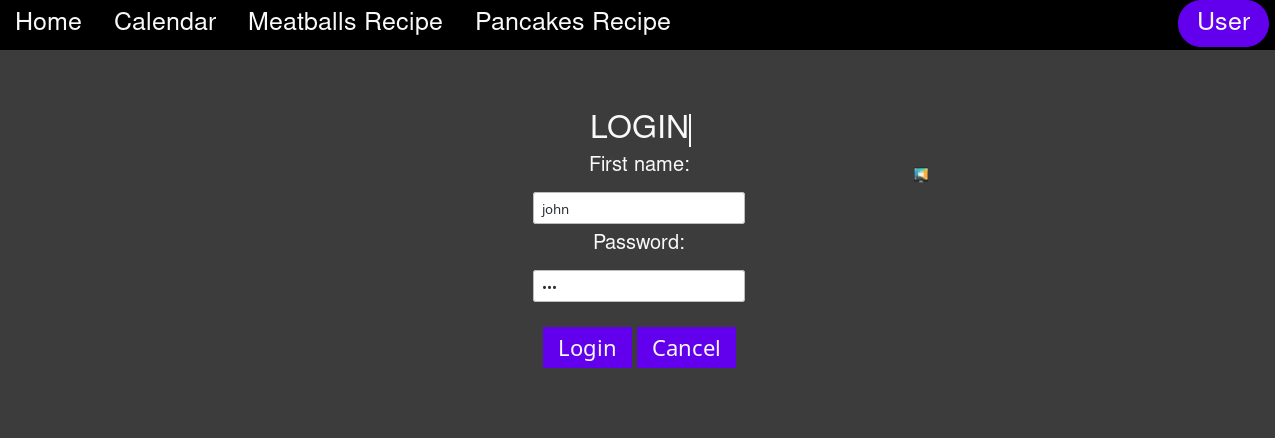
\includegraphics[scale=0.3]{images/login_form.png}
    \caption{A sample user interface screenshot to illustrate caption (this text), numbering and reference in text.}
    \label{fig:login_form}
  \end{center}
\end{figure}
As the form should not call PHP functions directly, it instead directs to a PHP file where execution starts from line 1. This option can be seen in \citet{kimblad_git_2019-php_call} where the form is linked to the file login.php.

Once the user has provided valid login information and the user has been logged in the user will be directed to a a personal user page welcoming the logged in users and also providing an option to log out. The login button in the navbar is also replaced with User button that redirects to this same page providing a log out option. This page can be seen in figure \ref{fig:user_page}. Once the user logs out they are redirected to the login page that provides a form for the username and password. 
\begin{figure}[h!]
  \begin{center}
    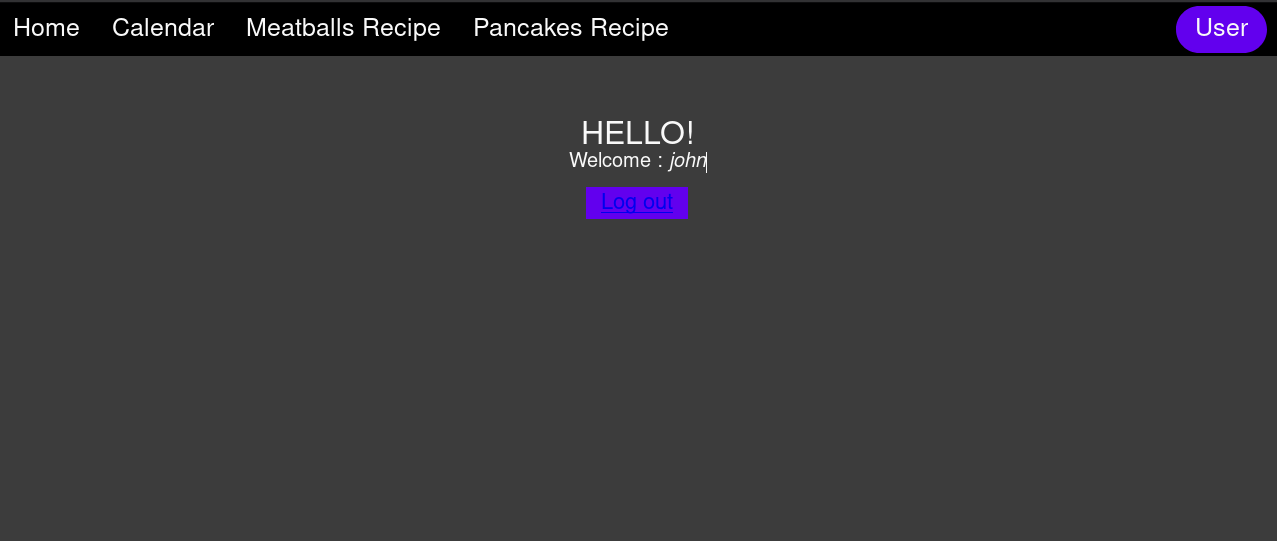
\includegraphics[scale=0.3]{images/user_page.png}
    \caption{A sample user interface screenshot to illustrate caption (this text), numbering and reference in text.}
    \label{fig:user_page}
  \end{center}
\end{figure}

The ability to write comments was added to the bottom of each recipe page and contains a html textarea that is used as input for the comment and a submit button. PHP is used to check if there is a logged in user, using the session variable, and if so shows the textarea and the button. If a comment is submitted by a user the information is sent as an SQL query to the connected database such that the comment is saved server-side. The textarea and submit button can be seen in figure \ref{fig:comment_form}. 

\begin{figure}[h!]
  \begin{center}
    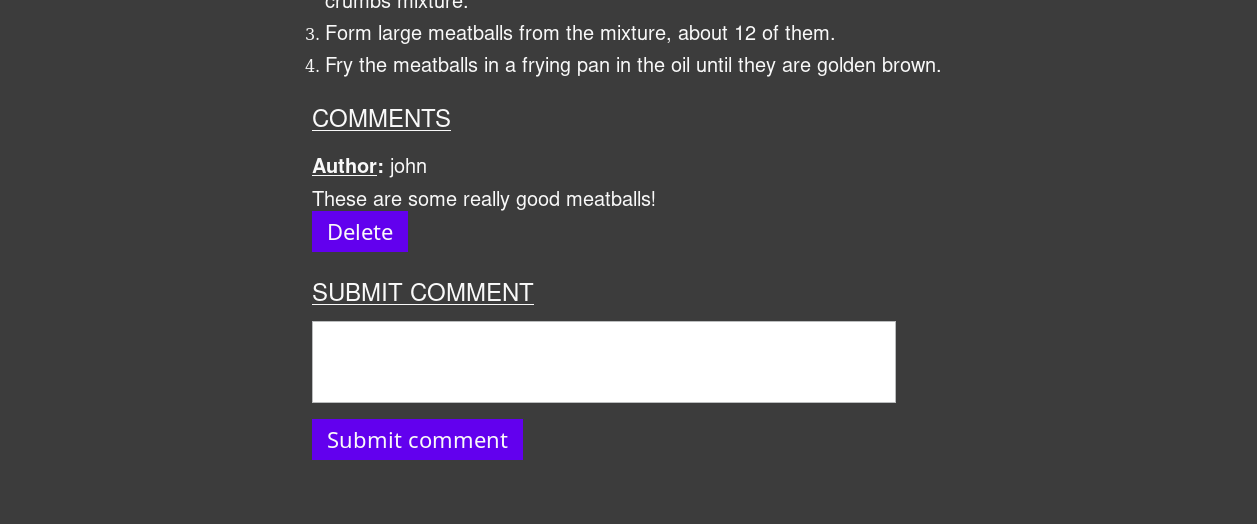
\includegraphics[scale=0.3]{images/comment_form.png}
    \caption{A sample user interface screenshot to illustrate caption (this text), numbering and reference in text.}
    \label{fig:comment_form}
  \end{center}
\end{figure}

Comments are listed under each recipe for all viewers of the page (including non logged in users). To have comments show up for specific recipes it is also saved in the database what page the comments were made on. This way it is made sure that comments are displayed on the relevant page. PHP is used to fetch the comments from the database and display the relevant HTML on the page. When iterating through each comment it is also checked if the creator of the comment is the same user as is logged in at the moment. If this is true, then a button to delete that specific comment is also shown on the page next below the relevant comment. The comment layout including the delete button can be seen in figure \ref{fig:comment_form}.
The PHP code fetching information from the database and presenting the information as HTML for specifically the meatballs recipe can be found at \citet{kimblad_git_2019-comments} and similar code with appropriate changes can also be found on the page presenting the pancakes recipe.

\section{Discussion}

The requirements can be summarised by the two parts they were divided up into in the introduction. The first part covers the login and user managemnt on the website. And has been shown using screenshots a log in form is provided on the website using HTML and CSS such that it also matches the rest of the design of the website. The form also associates each user with a username and a password. A link to the public Github repository has also been provided where it shows in code that the action of the html attribute is not set to a PHP function, but instead a URL. 

The five basic heuristics for interface design have also been taken into consideration during the design. Visibility of system status is provided by changing the login button in the navbar to a user button once logged in. By providing this in the navbar we also provide recognition rather than recall and an aesthetic and minimalist design. Match between systeam and the real world is considered by not using system-oriented terms, but instead terms that are intuitive to the user such as login, log out and user. 

The second part of the requirements covers the comment functionality on the recipe pages. The first requirement is that logged in users should be able to leave new comments on recipes which has been made possible using a database connected to the backend. The database also holds information about which recipe the comment belongs such that every comment is only shown on the relevant page. All users, wether logged in or not, are able to read all comments but only logged in users are able to delete comments that are their own. Commenting also follows the five basic heuristics for user interface design. Visibility of system status is used by not showing any of the commenting elements when the user is not logged in, there is a match between system and the real world by using intuitive terms such ass comment, delete comment, submit comment. Recognition rather than recall is handled by also making the design aesthetic and minimalist as there is no clutter, but each part of the page clearly has a unique purpose presented to the user.
%\nocite{*}
\printbibliography

\section{Comments About the Course}
Time spent on this assignment was approximately 40 hours. 

\end{document}
